\documentclass[landscape]{article}
\usepackage[a4paper,margin=3mm,landscape]{geometry}
\usepackage[scaled=0.92]{helvet}
\usepackage{multicol, multirow}
\usepackage{makecell}
\usepackage{array} 
\usepackage[table]{xcolor}
\usepackage{enumitem} 
\usepackage{amssymb}
\usepackage{graphicx}
\setlist{nosep}

\graphicspath{{./images/}}

\pdfinfo{
    /Title (CS2109S Cheatsheet.pdf)
    /Creator (TeX)
    /Producer (pdfTeX 1.40.0)
    /Author (Selwyn Ang)
    /Subject (CS2109S)
    /Keywords (CS2109S, Cheatsheet, NUS, Introduction to Artificial Intelligence and Machine Learning) 
}

% Turn off header and footer
\pagestyle{empty}


\makeatletter
\DeclareRobustCommand\smaller{\@setfontsize\smaller{6pt}{6.5pt}}
\makeatother

% redefine section commands to use less space
\makeatletter
\renewcommand{\section}{\@startsection{section}{1}{0mm}%
  {-0.1ex plus -0.1ex minus -0.1ex}%
  {0.1ex plus .1ex minus 0.1ex}%
{\normalfont\small\bfseries}}
\renewcommand{\subsection}{\@startsection{subsection}{2}{0mm}%
  {-0.1ex plus -0.1ex minus -0.1ex}%
  {0.1ex plus .1ex minus 0.1ex}%
{\normalfont\scriptsize\bfseries}}
\renewcommand{\subsubsection}{\@startsection{subsubsection}{3}{0mm}%
  {-0.1ex plus -0.1ex minus -0.1ex}%
  {0.1ex plus .1ex minus 0.1ex}%
{\normalfont\smaller\bfseries}}%
\makeatother



\renewcommand{\familydefault}{\sfdefault}
\renewcommand\rmdefault{\sfdefault}
%  makes nested numbering (e.g. 1.1.1, 1.1.2, etc)
\renewcommand{\labelenumii}{\theenumii}
\renewcommand{\theenumii}{\theenumi.\arabic{enumii}.}
\renewcommand\labelitemii{•}
\renewcommand\labelitemiii{•}

\setlength{\parindent}{0pt}
\setlength{\parskip}{0pt plus 0.5ex}
\setlength{\columnsep}{0.2cm}
%% adjust spacing for all itemize/enumerate
\setlength{\leftmargini}{0.5cm}
\setlength{\leftmarginii}{0.5cm}
\setlist[itemize,1]{leftmargin=2mm,labelindent=1mm,labelsep=1mm}
\setlist[itemize,2]{leftmargin=2mm,labelindent=1mm,labelsep=1mm}
\setlist[itemize,3]{leftmargin=2mm,labelindent=1mm,labelsep=1mm}
\setlist[enumerate,1]{leftmargin=2mm,labelindent=1mm,labelsep=1mm}
\setlist[enumerate,2]{leftmargin=2mm,labelindent=1mm,labelsep=1mm}
\setlist[enumerate,3]{leftmargin=2mm,labelindent=1mm,labelsep=1mm}

% tightcenter
\newenvironment{tightcenter}{%
  \setlength\topsep{0pt}
  \setlength\parskip{0pt}
  \begin{center}
    }{%
  \end{center}
}

% boxed
\newenvironment{tightbox}{%
  \setlength\topsep{0pt}
  \setlength\parskip{0pt}
  \begin{center}
    \begin{tabular}{|@{\hspace{\dimexpr\fboxsep+0.5\arrayrulewidth}}c@{\hspace{\dimexpr\fboxsep+0.5\arrayrulewidth}}|}
      \hline
    }
    {%
    \\ \hline
    \end{tabular}
  \end{center}
}

% fixed width box
\newenvironment{fixedbox}[1][0.7]{
  \setlength\topsep{0pt}
  \setlength\parskip{0pt}
  \begin{center}
    \begin{tabular}{|>{\centering\arraybackslash}m{#1\linewidth}|}
    \hline
  }{
  \\ \hline
  \end{tabular}
  \end{center}
}

% definition of a new term
\usepackage{soul}
\definecolor{paleyellow}{RGB}{251,243,218}
\newcommand{\definition}[2][]{\sethlcolor{paleyellow}\hl{\textbf{#2}} #1  $\rightarrow$}
% inline definition
\newcommand{\ildefinition}[1]{\sethlcolor{paleyellow}\hl{\textbf{#1}}}

% important note (attention)
\newcommand{\attention}{{\color{red}\textbf{! }}}

% nice proof
\newenvironment{niceproof}[1][Proof]
{%
  \sbox0{\textit{#1}. }%
  \list{}{\labelwidth\wd0 \leftmargin\wd0 \labelsep 0pt }
\item[\usebox0]}
  {\endlist}


\usepackage{color, soul}
\usepackage{listings}
\usepackage{inconsolata}

\definecolor{codegreen}{rgb}{0,0.6,0}
\definecolor{codegray}{rgb}{0.5,0.5,0.5}
\definecolor{codepurple}{HTML}{C42043}
\definecolor{backcolour}{HTML}{F2F2F2}
\definecolor{bookColor}{cmyk}{0,0,0,0.90}

\newcommand{\code}[1]{\texttt{\sethlcolor{backcolour}\hl{$\,$#1$\,$}}}

% SQL code blocks
% define SQL styles
\lstdefinestyle{mySQL}{%
  language=SQL,
  backgroundcolor=\color{backcolour},
  commentstyle=\color{codegreen},
  keywordstyle=\color{codepurple},
  numberstyle=\numberstyle,
  stringstyle=\color{codepurple},
  basicstyle=\scriptsize\ttfamily,
  breaklines=true,
}



% --------------------------------------------------------

\begin{document}
\raggedright
\tiny
\begin{multicols*}{5}
    \setlength{\columnseprule}{0.25pt}

    \begin{tightcenter}
        \fbox{%
          \parbox{0.8\linewidth}{\centering \textcolor{black}{
              {\Large\textbf{CS2109S Midterms}}
            \\ \normalsize{AY24/25 SEM 1}}
            \\ {\footnotesize \textcolor{gray}{github/SelwynAng}}
          }%
        }
    \end{tightcenter}
    
    \section{Introduction to AI}
    \subsection{Intelligent Agents}
    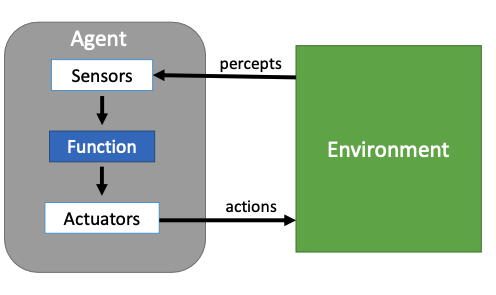
\includegraphics[width=0.7\linewidth]{1_PEAS.jpg}
    \begin{itemize}
      \item \textbf{PEAS} 
      \begin{enumerate}
        \item \underline{Performance Measure:} Best for whom, what are we optimizing, what information is available, any unintended effects, what are the costs 
        \item \underline{Environment:} Refer to Environment section
        \item \underline{Actuators:} Allow intelligent agent to take actions or affect its environment
        \item \underline{Sensors:} Allow intelligent agent to perceive information about its environment 
      \end{enumerate}
      \item \textbf{Agent Function:} Maps from percept histories to actions, refer to Agent Function section
    \end{itemize}
    
    \subsection{Task Environment}
    \begin{enumerate}
      \item \textbf{Fully Observable VS Partially Observable}
      \begin{itemize}
        \item \underline{Fully Observable:} Agent has complete \& accurate info about env state at all times (Eg. Chess)
        \item \underline{Partially Observable:} Agent has access to incomplete, uncertain or noisy info about env state (Eg. Self-driving cars)
      \end{itemize}
      \item \textbf{Deterministic VS Stochastic VS Strategic}
      \begin{itemize}
        \item \underline{Deterministic:} Next env state is completely determined by current state \& agent action $\vert$ Outcome is fully predictable (Eg. Sudoku)
        \item \underline{Stochastic:} Next env state is not completely determined by current state \& agent action $\vert$ Outcome is uncertain (Eg. Self-driving car)
        \item \underline{Strategic:} Env is deterministic, but outcomes depend on other agents' actions, requiring agent to consider strategies \& behaviors of others (Eg. Chess)
      \end{itemize}
      \item \textbf{Episodic VS Sequential}
      \begin{itemize}
        \item \underline{Episodic:} Agent actions are divided into discrete periods, each episode is independent of one another, agent makes decisions based on current episode (Eg. Classification task)
        \item \underline{Sequential:} Agent actions are inter-dependent, each action affects future states \& decisions, agent considers sequence of actions over time (Eg. Chess)
      \end{itemize}
      \item \textbf{Static VS Dynamic}
      \begin{itemize}
        \item \underline{Static:} Env state does not change while agent is deliberating
        \item \underline{Dynamic:} Env state changes over time even when agent is deliberating
        \item \underline{Semi-dynamic:} Env state does not change, but agent's performance score does
      \end{itemize}
      \item \textbf{Discrete VS Continuous}
      \begin{itemize}
        \item \underline{Discrete:} Finite \# of distinct, clearly defined percepts \& actions
        \item \underline{Continuous:} Infinite \# of percepts \& actions
      \end{itemize}
      \item \textbf{Single Agent VS Multi Agent}
      \begin{itemize}
        \item \underline{Single Agent:} Agent operating by itself in an env
        \item \underline{Multi Agent:} Multiple agents in an env
      \end{itemize}
    \end{enumerate}

    \subsection{Agent Structures}
    \textit{Note: Agent is completely specified by Agent Function mapping percept sequences to actions}
    \begin{enumerate}
      \item \textbf{Simple Reflex Agent:} Operates based on a set of predefined rules or conditions $\rightarrow$ Reacts to current state of env with a corresponding action $\rightarrow$ Does not have memory of past states or actions \& does not consider future consequences
      \item \textbf{Model-based Reflex Agent:} Extends simple reflex agent by maintaining internal model of world $\rightarrow$ Allows agent to keep track of current env state \& handle situations where env state is partially observable or changes over time
      \item \textbf{Goal-based Agent:} Operates with specific goals in mind $\rightarrow$ Selects actions based on ability to achieve these goals $\rightarrow$ Considers future \& plans its actions to achieve desired end state $\vert$ Uses goal representation \& perform search and planning
      \item \textbf{Utility-based Agent:} Extends goal based agent by considering not just whether goals are achieved, but how well they are achieved $\rightarrow$ Assigns utility value to different states \& chooses actions that maximize overall utility
      \item \textbf{Learning Agent:} Improves performance over time by learning from its experiences $\vert$ Can be reflex, model, goal \& utility based
    \end{enumerate}
    \begin{itemize}
      \item \textbf{Exploitation:} Maximize expected utility according to current knowledge about world
      \item \textbf{Exploration:} Trying to learn more about the world
    \end{itemize}

    \section{Solving Problems by Searching}
    \subsection{Designing an Agent}
    \begin{itemize}
      \item \textbf{Assumptions:} Goal-based agent $\vert$ Env is fully observable, deterministic, static, discrete
      \item \textbf{Problem-solving Agent:} Agent that plans ahead (considers a seq. of actions that form a path to a goal state), undertakes SEARCH process
      \item \textbf{Steps:}
      \begin{enumerate}
        \item \underline{Goal Formulation:} \textit{(What do we want?)}
        \item \underline{Problem Formulation:} \textit{(How the world works?)} $\rightarrow$ States (state space), Initial State(initial state of agent), Goal State/Test (goal state of agent), Actions (things that agent can do in a given state), Transition Model (specifies outcome of an action to a given state \& how it leads to new states), Action Cost Function (cost of performing an action)
        \item \underline{Search:} \textit{(How to achieve it?)} $\rightarrow$ Path (seq. of actions), Solution (path to a goal)
        \item \underline{Execute}
      \end{enumerate}
      \item \textbf{Representation Invariant:} A condition that must be true over all valid concrete representations of a class
    \end{itemize}

    \subsection{Search Algorithms (Introduction)}
    \begin{itemize}
      \item \textbf{Search Algorithm:} Takes in search problem (input), returns solution/failure (output) $\vert$ Defined by Order of Expansion (FRONTIER)
      \item \textbf{Evaluation Criteria:}
      \begin{enumerate}
        \item \underline{Time Complexity:} \# of nodes generated/expanded
        \item \underline{Space Complexity:} Max \# of nodes in memory
        \item \underline{Completeness:} Does it return solution if it exists?
        \item \underline{Optimality:} Does it always find least cost solution?
      \end{enumerate}
      \begin{multicols}{2}
        \textbf{Tree Search:} 
        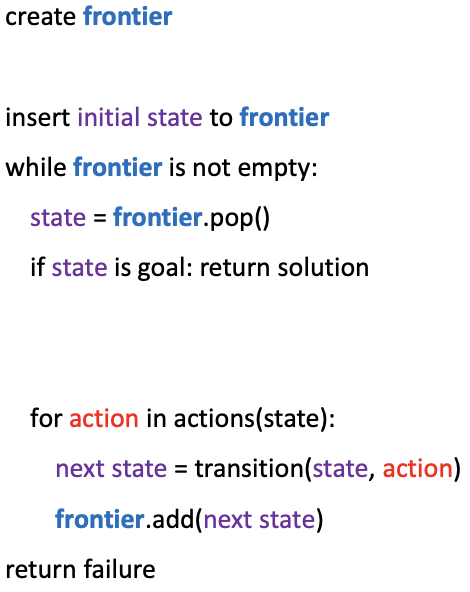
\includegraphics[width=0.75\linewidth]{2_tree_search.png}
        \\
        \columnbreak
        \textbf{Graph Search:}
        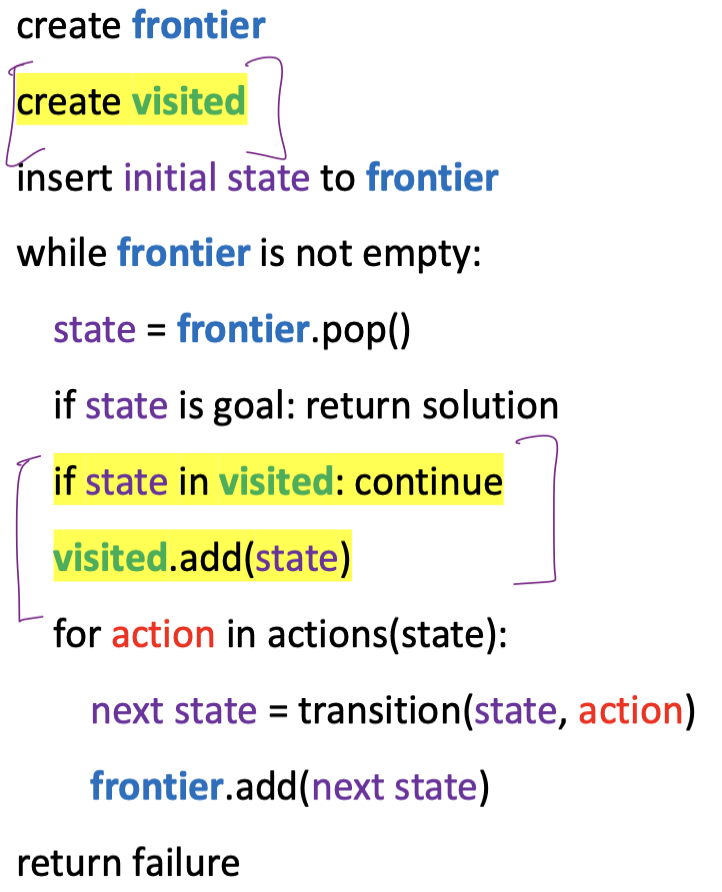
\includegraphics[width=0.75\linewidth]{3_graph_search.png}
      \end{multicols}
      \item \textbf{Checking of Goal State:}
      \begin{itemize}
        \item New state is checked for goal state before new states are PUSHED to frontier $\rightarrow$ Expand less states, may skip states with less cost
        \item State is checked for goal state after state is POPPED from frontier $\rightarrow$ Expand more states, will not skip states with less cost
      \end{itemize}
    \end{itemize}

    \subsection{Search Algorithms (Uninformed Search)}
    \begin{itemize}
      \item \textbf{Key Idea:} Search Algo is given no clue about how close a state is to the goal $\vert$ Can be Tree or Graph Search
      \item \textbf{BFS:} Queue Frontier $\vert$ Time Complexity: $O(b^d) = 1 + b + b^2 +$ $... + b^d$, where $b$ is branching factor, $d$ is depth of optimal solution $\vert$ Space Complexity: $O(b^d)$ when expanded until last child in worst case $\vert$ Completeness: Complete if $b$ is finite $\vert$ Optimality: Optimal if step cost is same everywhere
      \item \textbf{UCS:} Priority Queue (path cost) Frontier, where path cost == cost from root to a state $\vert$ Time Complexity: $O(b^{C^*/\epsilon})$, where $C^*$ is cost of optimal solution, $\epsilon$ is minimum edge cost $\rightarrow$ $C^*/\epsilon$ is est. depth of optimal solution in worst case $\vert$ Completeness: Complete if $\epsilon > 0$ and $C^*$ is finite (if $\epsilon = 0$, zero cost cycle may occur) $\vert$ Optimality: Optimal if $\epsilon > 0$
      \textit{Note: BFS is special case of UCS where step cost == 1 for every edge}
      \item \textbf{DFS:} Stack Frontier $\vert$ Time Complexity: $O(b^m)$ where $b$ is branching factor, $m$ is max depth $\vert$ Space Complexity: $O(bm)$ as only 1 path is expanded at one time $\vert$ Completeness: Not complete (when depth is infinite or can go back or forth) $\vert$ Optimality: Not optimal (there can be paths with less cost not explored yet)
      \item \textbf{DLS (Depth Limited Search):} Limit the search depth to $l$ where $l<=m$, backtrack once depth limit is reached $\vert$ Time Complexity: $O(b^l)$ $\vert$ Space Complexity: $O(bl)$ $\vert$ Completeness: Not complete when soln lies deeper $l$ $\vert$ Optimality: Not optimal when soln lies deeper than $l$
      \textit{Note: We dk the depth of solution, which is a downside}
      \item \textbf{IDS (Iterative Deepening Search):} Do DLS with max depth of $0,..,\infty$ $\rightarrow$ return soln if found, otherwise increase depth $\vert$ Time Complexity: $O(b^d)$, $Overhead=(n_{IDS} - n_{DLS})/n_{DLS}$ $\vert$ Space Complexity: $O(bd)$ $\vert$ Completeness: Complete $\vert$ Optimality: Optimal if step cost is same everywhere \\
      \textit{Note: IDS is not always faster than DFS $\rightarrow$ Consider state space s.t. each state have only single successor \& goal node is at depth $n$ $\rightarrow$ IDS will run in $O(n^2)$, DFS will run in $O(n)$}
      \item \textbf{Backward Search:} Search from goal
      \item \textbf{Bidirectional Search:} Combine forward search \& backward search, stop when 2 searches meet $\vert$ Time Complexity: $2*O(b^{d/2}) < O(b^d)$
    \end{itemize}

    \subsection{Search Algorithms (Informed Search)}
    \begin{itemize}
      \item \textbf{Key Idea:} Search Algo has a clue on how close a state is to the goal
      \item \textbf{Best First Search:} Priority Queue ($f(n)$) Frontier, where $f(n)$ estimates the goodness of a state (Node with lowest $f(n)$ is selected first to be expanded) $\vert$ $f(n)$ can be purely heuristic (estimated cost from $n$ to goal) or a combi of path cost \& heuristic
      \item \textbf{Greedy Best First Search:} Priority Queue ($f(n) = h(n)$) Frontier, where $h(n)$ is heuristic function that est. cost from $n$ to goal (Expands node that seems closest to goal according to $h(n)$ without considering path cost so far) $\vert$ Time Complexity: $O(b^m)$ $\vert$  Space Complexity: $O(b^m)$ $\vert$ Completeness: Not complete since GBFS might keep expanding nodes based on $h(n)$ without ever finding goal $\vert$  Optimality: Not optimal since GBFS selects nodes based on $h(n)$ without considering path cost
      \item \textbf{$A^*$ Search:} Priority Queue ($f(n) = g(n) + h(n)$) where $g(n)$ is cost so far to reach $n$ $\vert$ Time Complexity: $O(b^m)$ $\vert$ Space Complexity: $O(b^m)$ $\vert$  Completeness: Complete $\vert$ Optimality: Optimal
      \begin{itemize}
        \item If $h(n)$ is admissible $\rightarrow$ $A^*$ using Tree search is optimal
        \item If $h(n)$ is consistent $\rightarrow$ $A^*$ using Graph search is optimal
        \item \textit{Note: UCS is special case of $A^*$ search where $h(n) = 0$}
      \end{itemize}

      \subsection{Heuristics}
      \begin{itemize}
        \item Estimate cost from node $n$ to goal
        \item \textbf{Admissible Heuristics:} For every node $n$, $h(n) \leq h^*(n)$, where $h^*(n)$ is true cost to reach goal state from $n$ (Never over-estimate)
        \item \textbf{Consistent Heuristics:} For every node $n$, every successor $n'$ generated by action $a$, $h(n) \leq c(n,a,n') + h(n')$ and $h(G) = 0$ (Proof $h(n) - h(n') \leq c(n,a,n')$) \\
        \textit{Note: If $h(n)$ is consistent, $f(n') \geq f(n)$ $\rightarrow$ $f(n)$ is non-decreasing along any path $\rightarrow$ Nodes are expanded in order of increasing $f$ cost}
        \item \textbf{Dominance:} If $h_2(n) \geq h_1(n)$ for all $n$ $\rightarrow$ $h_2$ dominates $h_1$ $\vert$ If $h_2$ is admissible $\rightarrow$ $h_2$ is better for search
        \item \textbf{Creating Admissible Heuristics:}
        \begin{itemize}
          \item Problem with fewer restrictions on actions is called a relaxed problem
          \item Cost of an optimal soln to a relaxed problem is an admissible $h$ for original problem
        \end{itemize}
      \end{itemize}
    \end{itemize}

    \section{Local Search \& Adversarial Search}
    \subsection{Local Search}
    \begin{itemize}
      \item \textbf{Assumptions:} Agent is a Goal/Utility-based agent, Env has a very large state space
      \item \textbf{Informed \& Uninformed Search VS Local Search}
      \begin{enumerate}
        \item \underline{IUS:} Low to moderate state space $\vert$ Optimal or no soln $\vert$ Search path is usually the soln
        \item \underline{LS:} Very large state space $\vert$ Good enuf soln is preferable rather than no soln $\vert$ State is the soln (don't care about search path)
      \end{enumerate}
      \item \textbf{Local Search Overview:}
      \begin{itemize}
        \item \underline{Basic Idea:} Start somewhere in state space, move towards a better spot
        \item \underline{Problem Formulation:} States(state space), Initial State(initial state of agent), Goal test (optional, coz we actually dk the goal state, rely on eval function instead), Successor Function (possible states from a state), Evaluation Function (Output value/goodness of a state)
      \end{itemize}
      \item \textbf{Hill Climbing Algorithm}
      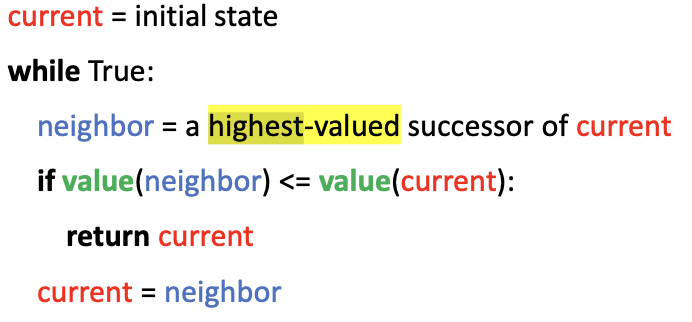
\includegraphics[width=0.75\linewidth]{4_hillclimbing.png}
      \begin{itemize}
        \item Known as Greedy Local Search (pick best amongst neighbors, repeat)
        \item \underline{Best Soln:} State space where eval. function has a max value (global max)
        \item \underline{Disadvantages:} Cannot reach global max if it enters local max, plateau $\vert$ Sensitive to choice of initial state, poor initial state may result in poor final state (Can overcome with random restarts, walks)
      \end{itemize}
      \item \textbf{Simulated Annealing}
      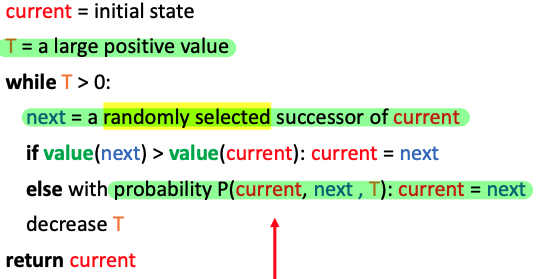
\includegraphics[width=0.75\linewidth]{5_simulated_annealing.png}
      \begin{itemize}
        \item P(current, next, T) = $e^{(value(next) - value(current))/T}$
        \item More exploration of bad states is allowed when $T$ is high, more exploitation is done when $T$ is low $\rightarrow$ basically choosing worse successor may lead to a better max
        \item \underline{Theorem:} If $T$ decreases slowly enough, SA will find global optimum with high probability
      \end{itemize}
    \end{itemize}

    \subsection{Adversarial Search}
    \begin{itemize}
      \item \textbf{Assumptions:} Agent is Utility-based $\vert$ Env is a game (game cannot be single player, partially observable, stochastic, but must be fully observable, deterministic, discrete, terminal states exist, 2 players, zero-sum, turn taking)
      \item \textbf{Minimax Algorithm:}
      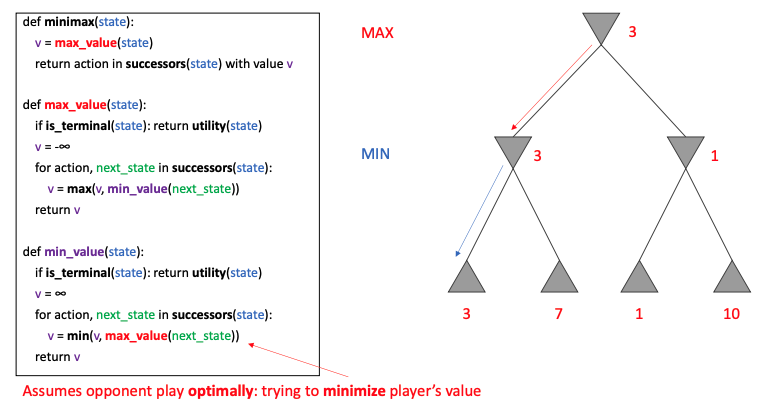
\includegraphics[width=0.9\linewidth]{6_minimax.png}
      \begin{itemize}
        \item \underline{Intuition:} MAX wins when utility is high, MIN wins when utility is low $\vert$ Assign utility values to all terminal states \& start tracing from terminal states $\rightarrow$ Eventually, all states will have utility values, starting player can choose a state that will max/min his utility
        \item \underline{Analysis:} Completeness: Complete if tree is finite $\vert$ Time Complexity: $O(b^m)$ $\vert$ Space Complexity: $O(bm)$ depth first exploration $\vert$ Optimality: Optimal against optimal opponent
      \end{itemize}
      \item \textbf{Alpha-beta Pruning}
      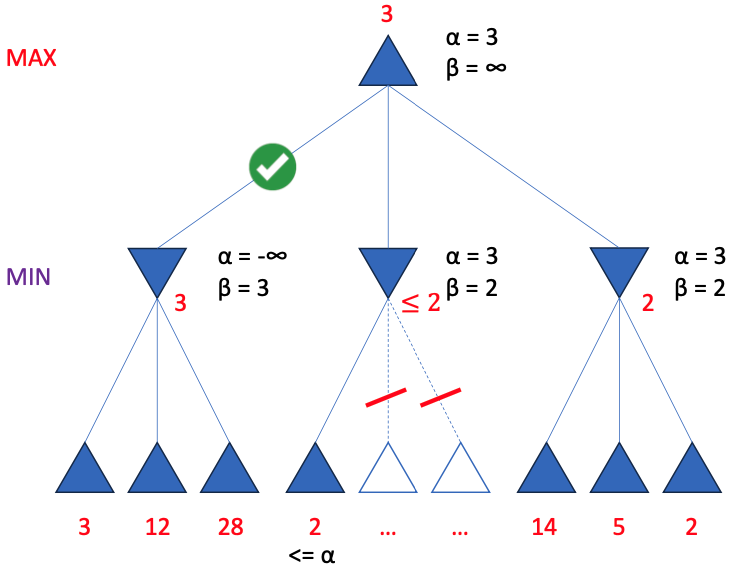
\includegraphics[width=0.75\linewidth]{7_alphabeta.png}
      \begin{itemize}
        \item \underline{Definitions:} $\alpha$ is best explored option to the root for MAX player (Highest value for MAX) $\vert$ $\beta$ is best explored option along path to the root for MIN player (Lowest value for MIN)
        \item \underline{Procedure:} 1. Assign $\alpha = -\infty, \beta = \infty$ for root 2. Propagate values down to the terminal node 3. Update $\alpha$ value at MAX node, $\beta$ value at MIN node 4. Propagate values up 5. Prune branches of nodes where $\alpha \geq \beta$
      \end{itemize}
      \item \textbf{Minimax with Cutoff}
      \begin{itemize}
        \item Instead of calling $is\_terminal$, call $is\_cutoff$ which returns TRUE if (1): State is terminal or (2): Cut-off is reached
        \item Instead of using $utility$, call $eval$ which is an eval. function that returns (1): Utility for terminal states or (2): Heuristic value for non-terminal states
      \end{itemize}
    \end{itemize}

    \section{Introduction to ML \& Decision Trees}
    \subsection{Introduction to ML}
    \begin{itemize}
      \item \textbf{Definitions:} Computer program is said to learn from experience $E$ w.r.t. some class of tasks $T$ \& performance measure $P$, if its performance at tasks in $T$, as measured by $P$, improves with experience $E$
      \item \textbf{Types of Feedback:}
      \begin{enumerate}
        \item \underline{Supervised Learning:} Involves training a model on a labeled dataset, where input data is paired with correct output $\rightarrow$ Model learns to map inputs to outputs based on this labeled data, allowing it to make predictions on new data
        \begin{itemize}
          \item \underline{Regression:} Predict continuous input
          \item \underline{Classification:} Predict discrete input
        \end{itemize} 
        \item \underline{Unsupervised Learning:} Deals with dataset that do not have labeled outputs $\rightarrow$ Goal is to identify patterns \& structures within data
        \item \underline{Reinforcement Learning:} Agent learns to make decisions by interacting with an environment $\rightarrow$ Agent receives feedback in the form of rewards or penalties based on its actions $\rightarrow$ Learns optimal behaviors over time
      \end{enumerate}
      \item \textbf{Formal Definitions:}
      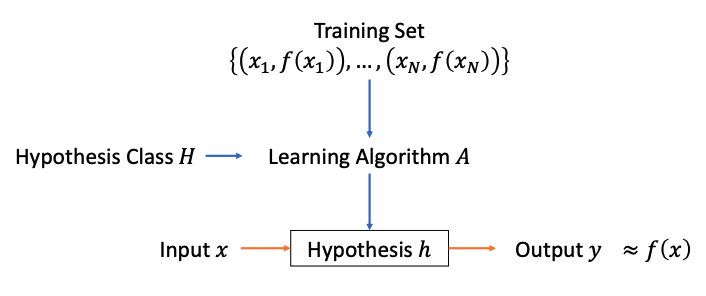
\includegraphics[width=0.75\linewidth]{8_ml_formal.png}
    \end{itemize}

    \subsection{Performance Measure}
    \begin{itemize}
      \item \textbf{Regression:} \\
      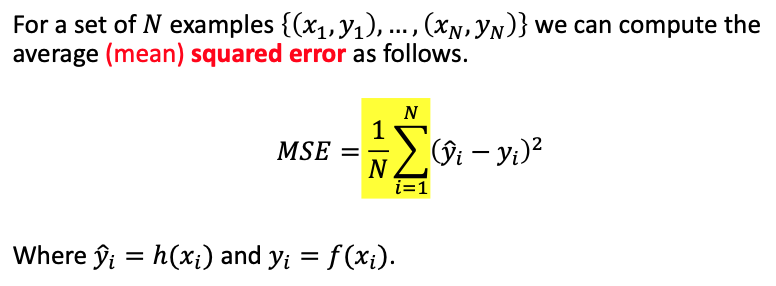
\includegraphics[width=0.75\linewidth]{9_mse.png}
      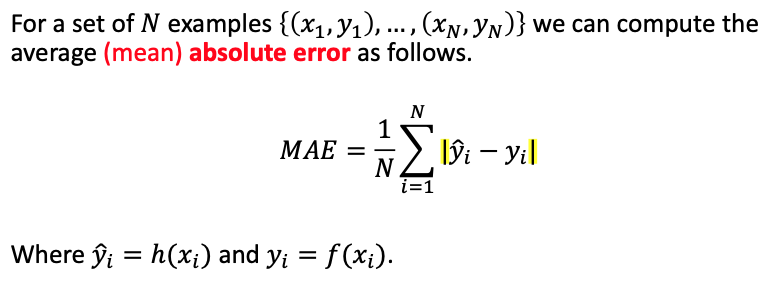
\includegraphics[width=0.75\linewidth]{10_mae.png}
      \item \textbf{Classification:} \\
      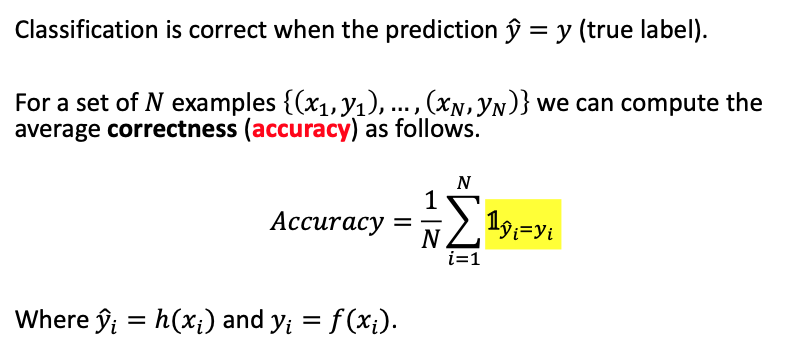
\includegraphics[width=0.75\linewidth]{11_accuracy.png}
      \begin{multicols}{2}
        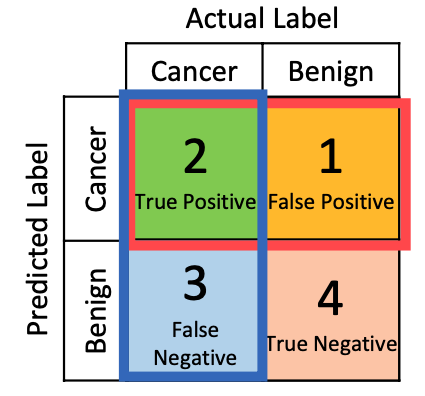
\includegraphics[width=0.8\linewidth]{12_confusion_matrix.png}
        \\
        \columnbreak
        \begin{itemize}
          \item \textbf{Accuracy:} $\frac{TP+TN}{TP+FN+FP+TN}$
          \item \textbf{Precision:} $\frac{TP}{TP+FP}$ (How many selected items are relevant, maximise if FP is costly)
          \item \textbf{Recall:} $\frac{TP}{TP+FN}$ (How many relevant items are selected, maximise if FN is dangerous)
        \end{itemize}
      \end{multicols}
      \item \textbf{F1 Score:} $\frac{2}{1/precision + 1/recall}$
    \end{itemize}
    
    \subsection{Decision Trees}
    \begin{itemize}
      \item \textbf{Traits of Decision Trees:}
      \begin{itemize}
        \item Decision Trees can express any function of input attributes
        \item Consistent Decision Tree for any training set, but probably will not generalize to new examples
        \item \underline{\# of distinct decision trees with $n$ boolean attributes} = $2^{2^n}$
      \end{itemize}
      \item \textbf{Decision Tree Learning Algorithm}
      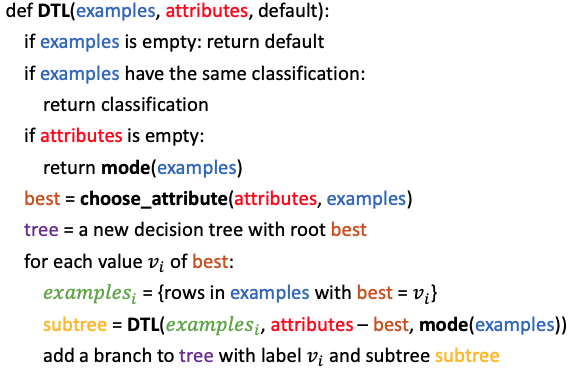
\includegraphics[width=0.8\linewidth]{13_decision_tree.png}
      \begin{itemize}
        \item \underline{mode:} Category with the highest number
        \item \underline{choose attribute:} Chooses attribute with the highest information gain
      \end{itemize}
      \item \textbf{Choosing an attribute:}
      \begin{itemize}
        \item Ideally select an attribute that splits examples into "all positive" or "all negative"
        \item \underline{Entropy} (Measure of randomness): $I(P(v_1),...,P(v_n)) = - \sum_{i=1}^{n}P(v_i)log_2P(v_i)$, where for data set containing $p$ positive \& $n$ negative examples, $I(\frac{p}{p+n}, \frac{n}{p+n}) = -\frac{p}{p+n}log_2\frac{p}{p+n}-\frac{n}{p+n}log_2\frac{n}{p+n}$ \\
        \textit{Note: I(1,0) = I(0,1) = 0}
        \item \underline{Information Gain} (Entropy of curr. node - Total Entropy of children nodes): $IG(A) = I(\frac{p}{p+n}, \frac{n}{p+n}) - remainder(A)$ \\
        remainder(A) = $\sum_{i=1}^{v} \frac{p_i+n_i}{p+n} I(\frac{p_i}{p_i+n_i}, \frac{n_i}{p_i+n_i})$, where examples are split into $v$ subsets by attribute $A$
      \end{itemize}
      \item \textbf{Dealing with continuous valued attributes:} Define a discrete valued input attribute to partition values into discrete set of intervals
      \item \textbf{Dealing with missing values:} Assign most common value of attribute, assign probability to each value and sample, drop attribute, drop rows
      \item \textbf{Overfitting:} Decision Tree is perfect on training data, but worse on test data
      \item \textbf{Occam Razor:} Prefer short/simple hypothesis (long/complex hypothesis that fits data may be coincidence)
      \item \textbf{Pruning:} Prevents nodes from being split even when it fails to cleanly separate examples (Min samples leaf: Merge until leaf node is above min. samples number $\vert$ Max depth: Merge until leaf nodes are at depth less than max depth)
    \end{itemize}
  \end{multicols*}
\end{document}
